\clearpage



\section{Flashback}

\subsection{氧化性顺序}

\paragraph{氧化性}

$$
\ce{F2} > \ce{O2} > \ce{Cl2} > \ce{Br2} > \ce{Fe^3+} > \ce{I2} > \ce{S}
$$

$$
\ce{F-} < \ce{H2O} < \ce{Cl-} < \ce{Br-} < \ce{Fe^2+} < \ce{I-} < \ce{S^2-} < \text{惰性电极}
$$

\paragraph{还原性}

\subparagraph{金属活动顺序表}

\begin{itemize}
	\item 钾钙钠镁铝:\ce{K} Ca Na Mg Al
	\item 锌铁锡铅氢:Zn Fe Sn Pb H
	\item 铜汞银铂金:Cu Hg Ag Pt Au
\end{itemize}

$$
\ce{K} > \ce{Ca} > \ce{Na} > \ce{Mg} > \ce{Al} > \ce{Zn} > \ce{Fe} > \ce{Sn} > \ce{Pb} > \ce{H+} > \ce{Cu} > \ce{Hg} > \ce{Ag} > \ce{Pt} > \ce{Au}
$$

$$
\ce{K+} < \ce{Ca^2+} < \ce{Na+} < \ce{Mg^2+} < \ce{Al^3+} < \ce{H2O} < \ce{Zn^2+} < \ce{Fe^2+} < \ce{Sn^2+} < \ce{Pb^2+} < \ce{H+} < \ce{Cu+} < \ce{Hg+} < \ce{Fe^3+} < \ce{Ag+} < \ce{AuCl4-}
$$

\subsection{元素氧化图解}

\begin{figure}[h]
	\centering
	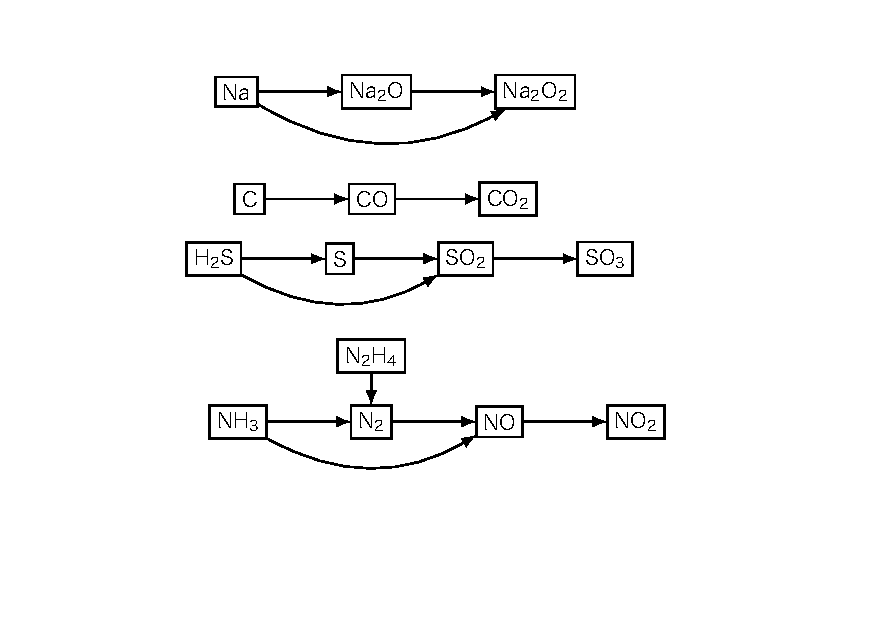
\includegraphics[scale=0.8]{res/Redox.pdf}
\end{figure}
